\documentclass[conference]{IEEEtran}
\IEEEoverridecommandlockouts
\usepackage[utf8]{inputenc}
\usepackage[T1]{fontenc}
\usepackage{amsmath,amssymb,amsfonts}
\usepackage{graphicx}
\usepackage{booktabs}
\usepackage{multirow}
\usepackage{url}
\usepackage{cite}
\usepackage[hidelinks]{hyperref}

% \tabinput reads a table body inside a tabular (plain \input breaks \bottomrule)
\makeatletter\newcommand{\tabinput}[1]{\@@input #1 }\makeatother

\begin{document}

\title{Confidence-Aware Graph Convolutional Networks\\ for Social Bot Detection: A Message-Passing\\ Reweighting Approach}

\author{\IEEEauthorblockN{Kanalbay Kassymkhan}
\IEEEauthorblockA{School of Software Engineering\\
Astana IT University\\
Astana, Kazakhstan\\
255479@astanait.edu.kz}}

\maketitle

\begin{abstract}
Social bots distort engagement metrics, amplify disinformation, and erode trust in online discourse, which motivates graph-based detectors that exploit relational structure. Standard Graph Convolutional Networks (GCNs) aggregate neighbor messages with weights that depend only on node degree, so a neighbor with a confident, well-separated prediction contributes exactly as much as one with a noisy, borderline prediction. We propose a Confidence-Aware GCN that reweights message passing by the model's own predictive confidence in each neighbor, computed as the maximum softmax probability from the previous epoch and renormalized over each node's incoming edges. The mechanism adds no learnable parameters and is implemented as a custom PyTorch Geometric layer. We verify it on a synthetic social graph (500 nodes) and evaluate it on a labeled Twitter bot dataset (5\,000-account subsample, cosine-similarity $k$-NN graph) against MLP, GCN, GraphSAGE and GAT baselines with 5-fold cross-validation repeated over 5 seeds, paired Wilcoxon tests with Holm correction, threshold-independent metrics, a threshold-matched comparison and ten ablations. The precision gain seen in an earlier single-split experiment (+3.0 points) does not survive this protocol: Conf-GCN matches GCN in precision (0.732 vs.\ 0.731, $p=0.83$) but loses 0.9 F1 points and 2.5 AUROC points, and at matched recall GCN is slightly \emph{more} precise. Uniform, shuffled and inverted confidences reproduce the full model to within one F1 point, showing that the effect comes from the change of normalization and the missing self-loop, not from confidence; on real data the confidence weights deviate from mean aggregation by only 6.5\% on average. Graph construction matters far more: on the description-only graph (edge homophily 0.62) every GCN-type model is beaten by a feature-only MLP (F1 0.807), whereas a $k$-NN graph over descriptions and metadata (homophily 0.76) lifts all GNNs above the MLP (F1 0.814--0.825). We report these negative and positive findings, release all code, and discuss when confidence weighting could still be useful.
\end{abstract}

\begin{IEEEkeywords}
bot detection, graph convolutional network, message passing, confidence weighting, node classification, negative results
\end{IEEEkeywords}

\section{Introduction}

Social media platforms increasingly contend with coordinated inauthentic accounts, commonly called social bots, that inflate follower counts, manufacture trending topics, and propagate disinformation at scale \cite{cresci2020decade}. Bots frequently operate in coordinated clusters and use templated, repetitive language, so both the relational structure of a social graph and the semantic content of posts carry complementary signal. This has motivated a shift from per-account classifiers toward Graph Neural Networks (GNNs), which propagate information along follow, mention, reply, or content-similarity edges and can therefore detect coordinated behavior invisible to a single-account feature vector.

A standard GCN \cite{kipf2017gcn} aggregates each node's neighborhood with degree-normalized weights that are agnostic to how reliable a neighbor's representation currently is. In bot detection this is a potential weakness: when bots are deliberately disguised to resemble genuine users, a small number of cross-class edges connect bot clusters to the human subgraph, and an ambiguous account near the decision boundary then contributes to its neighbors' updates with the same weight as an account classified with near-certainty. Noisy, low-confidence signal can thus leak across the class boundary.

This paper studies a Confidence-Aware GCN that addresses this weakness at the message-passing level. Each neighbor's contribution is scaled by the model's own confidence in that neighbor's class prediction from the previous epoch, renormalized so incoming weights sum to one. The mechanism requires no additional learnable parameters. In an earlier single-split experiment \cite{kassymkhan2026conf} the method raised precision by 3.0 points at a 7.6-point recall cost. Here we test whether that trade-off is a genuine effect of the confidence signal.

\textbf{Research questions.} \textbf{RQ1}: does the mechanism behave correctly (convergence; equivalence to uniform aggregation when all confidences are equal)? \textbf{RQ2}: how does it change accuracy, precision, recall, F1, AUROC and AUC-PR relative to GCN, GraphSAGE, GAT and a feature-only model, and is the change statistically reliable? \textbf{RQ3}: is the effect attributable to the confidence signal itself, rather than to the change in normalization or to a shift of the decision threshold? \textbf{RQ4}: how much does the construction of the similarity graph matter compared with the aggregation rule?

\textbf{Contributions.} (1) A parameter-free confidence-weighted message-passing layer, implemented as a custom PyTorch Geometric \texttt{MessagePassing} module, with unit tests for its formal properties. (2) A correctness validation on a synthetic social graph with known ground truth. (3) An evaluation on a real labeled Twitter dataset with repeated cross-validation, paired significance tests, stronger GNN baselines, a threshold-matched comparison and ten ablations that separate the confidence signal from its confounders. (4) A negative result: under this protocol the confidence signal has no measurable benefit, and we explain why (bounded, near-uniform weights). (5) A positive finding: graph construction decides whether any GNN beats a feature-only model on this tabular benchmark. Code, configurations and per-run results are public.\footnote{\url{https://github.com/solodancer235-star/confidence-aware-gcn-bot-detection}}

\section{Related Work}

\begin{table}[t]
\caption{Positioning relative to related aggregation schemes}
\label{tab:positioning}
\centering
\resizebox{\columnwidth}{!}{%
\begin{tabular}{@{}lccc@{}}
\toprule
Method & Weight source & Extra params & Uses pred.\ confidence\\
\midrule
GCN \cite{kipf2017gcn} & degree & no & no\\
GAT \cite{velickovic2018gat} & learned attention & yes & no\\
GraphSAGE \cite{hamilton2017sage} & mean/pool & yes & no\\
ConfGCN \cite{vashishth2019confgcn} & learned label confidence & yes & indirectly\\
Ours & softmax confidence & no & yes\\
\bottomrule
\end{tabular}}
\end{table}

\subsection{Feature-based bot detection}
Early detectors relied on hand-engineered behavioral and metadata features (posting frequency, account age, follower-to-friend ratios) combined with supervised classifiers; Botometer (formerly BotOrNot) blends a large number of such features in a supervised ensemble \cite{davis2016botornot}. Such approaches are effective against unsophisticated bots but degrade as bots adopt human-like patterns, and generalize poorly across datasets \cite{yang2020scalable,cresci2020decade}. Feature selection studies on Twitter bot detection show that profile and description features alone reach moderate accuracy \cite{lee2021discriminative}.

\subsection{Graph-based bot detection}
Graph-based approaches exploit the observation that bots, even when individually convincing, tend to be structurally distinguishable: they cluster densely, share near-duplicate content, or connect to common amplification targets. GCNs \cite{kipf2017gcn} and inductive GraphSAGE-style models \cite{hamilton2017sage} have been applied to spam and bot detection \cite{alhosseini2019detect}. BotRGCN and the Relational Graph Transformer extend this to heterogeneous graphs with multiple relation types \cite{feng2021botrgcn,feng2022rgt}, evaluated on the TwiBot-20 benchmark \cite{feng2021twibot20}. Graph Attention Networks (GATs) learn per-edge attention weights instead of fixing them to degree-based normalization \cite{velickovic2018gat}. The benefit of message passing depends strongly on homophily, i.e.\ the fraction of edges joining same-class nodes \cite{zhu2020beyond}.

\subsection{Confidence- and uncertainty-aware aggregation}
Several lines of work use model confidence. Pseudo-labeling and self-training use confident predictions on unlabeled data as additional supervision \cite{lee2013pseudo}. The closest graph-learning work is ConfGCN \cite{vashishth2019confgcn}, which estimates a per-node confidence over label distributions and uses it to modulate neighbor influence in semi-supervised node classification. Our approach differs in the signal and its cost: ConfGCN maintains a learned, per-node label-distribution estimate with additional parameters and a distribution-matching objective, whereas we derive confidence directly from the classifier's own softmax output, with no extra parameters, and study it specifically for bot detection. The reliability of softmax confidence itself is known to be imperfect and can be improved by calibration such as temperature scaling \cite{guo2017calibration}. Stochastic regularizers on message passing, such as DropEdge \cite{rong2020dropedge}, also aim to reduce the effect of noisy neighbors, but do so randomly and without regard to prediction reliability.

\subsection{Similarity graphs for tabular data}
Sentence-BERT embeddings \cite{reimers2019sbert} enable similarity-based edges between accounts posting near-duplicate content even without explicit social links. For tabular bot datasets that provide rich per-account metadata but no follow graph, a $k$-nearest-neighbor graph over embeddings is a common substitute for explicit structure, a construction long used in graph-based semi-supervised learning \cite{zhu2003semi}.

\section{Problem Formulation}

Let $G=(V,E)$ be a social graph, where $V$ is the set of accounts and $E$ the set of follow, mention, reply, or content-similarity edges. Each node $v$ has a feature vector $x_v\in\mathbb{R}^d$ built from a Sentence-BERT embedding of the account text concatenated with normalized profile metadata. A label $y_v\in\{0,1\}$ (0 = human, 1 = bot) is known for a subset of nodes. The task is transductive semi-supervised node classification: learn $f: G\rightarrow\{0,1\}^{|V|}$ predicting the label of every node, including those withheld from training, by propagating information along $E$.

\section{Methodology}

\subsection{Baseline GCN}
The baseline stacks three \texttt{GCNConv} layers (PyTorch Geometric) mapping $d\rightarrow64\rightarrow64\rightarrow2$, with ReLU and dropout ($p=0.5$). Node $i$ is updated at layer $l$ as
\begin{equation}
h_i^{(l+1)}=\sigma\Big(\sum_{j\in\mathcal{N}(i)\cup\{i\}}\frac{1}{\sqrt{\hat d_i\hat d_j}}\,W^{(l)}h_j^{(l)}\Big),
\label{eq:gcn}
\end{equation}
where $\hat d_i$ is the degree of $i$ including a self-loop. Training uses cross-entropy with Adam \cite{kingma2015adam}.

\subsection{Confidence-Aware GCN}
The confidence of node $j$ is the maximum softmax probability of its logits $z_j$ from the previous epoch:
\begin{equation}
c_j=\max_k\ \mathrm{softmax}(z_j)_k .
\label{eq:conf}
\end{equation}
For $C=2$ classes, $c_j\in[0.5,1]$. For every directed edge $j\rightarrow i$ the weight is renormalized over the incoming edges of $i$:
\begin{equation}
\tilde w_{j\rightarrow i}=\frac{c_j^{\alpha}}{\sum_{k\in\mathcal{N}(i)}c_k^{\alpha}},
\label{eq:weight}
\end{equation}
with $\alpha=1$ in the proposed model, and the node update becomes
\begin{equation}
h_i^{(l+1)}=\sigma\Big(\sum_{j\in\mathcal{N}(i)}\tilde w_{j\rightarrow i}\,W^{(l)}h_j^{(l)}\Big).
\label{eq:confupdate}
\end{equation}
Confidence is initialized to 1 for every node. At each epoch a forward pass produces logits for the loss and optimizer step; a second no-gradient forward pass in evaluation mode then recomputes the confidence vector for the next epoch. Confidence is stored as a plain tensor and updated inside a no-gradient context, so gradients never flow through it; this avoids a feedback loop between the loss and a quantity that depends on it. Confidence is computed from model outputs only and uses no labels, so evaluation nodes are not leaked.

\begin{table}[t]
\caption{Configuration of baseline and confidence-aware models}
\label{tab:config}
\centering
\resizebox{\columnwidth}{!}{%
\begin{tabular}{@{}lll@{}}
\toprule
Component & Baseline & Conf.-Aware\\
\midrule
Conv.\ layer & \texttt{GCNConv} (PyG) & \texttt{ConfWeightedConv}$^{*}$\\
Layers & 3 & 3\\
Hidden dim. & 64 & 64\\
Dropout & 0.5 & 0.5\\
Learnable params (Twitter) & 29\,570 & 29\,570\\
Optimizer & Adam (selected on val.) & Adam (selected on val.)\\
\bottomrule
\multicolumn{3}{@{}l}{\scriptsize $^{*}$Custom \texttt{MessagePassing} layer; mean-style normalization, no self-loop.}
\end{tabular}}
\end{table}

\subsection{Properties and limits of the mechanism}
\label{sec:props}
\textbf{Reduction to uniform aggregation.} When $c_j=1$ for all $j$ (the first forward pass), Eq.~\eqref{eq:confupdate} is mean aggregation over $\mathcal{N}(i)$. This is not identical to the symmetric degree normalization with self-loops used by the baseline (Eq.~\ref{eq:gcn}). The two models therefore differ in normalization and self-loop handling in addition to the confidence signal; we address this explicitly with ablations (Section~\ref{sec:ablations}) rather than assuming the difference is attributable to confidence alone. The layer is also invariant to a global rescaling of the confidences, since only ratios enter Eq.~\eqref{eq:weight}.

\textbf{Bounded influence.} Because $c_j\in[0.5,1]$ in the binary case, the weights of any two neighbors of the same node differ by at most a factor of $2^{\alpha}$. With $\alpha=1$ the mechanism can therefore only moderately rebalance a neighborhood; we measure how much it actually does in Section~\ref{sec:diag}.

\subsection{Architectural parity}
Both models use three layers, hidden dimension 64, dropout 0.5 and the same hyper-parameter search (Table~\ref{tab:config}); they have exactly the same number of learnable parameters (verified by a unit test). Parity of capacity does not imply that confidence is the only difference, so we complement it with the ablations below.

\section{Implementation}

The system is implemented in Python with PyTorch and PyTorch Geometric \cite{fey2019pyg}, sentence-transformers (\texttt{all-MiniLM-L6-v2}, 384-dimensional output) \cite{reimers2019sbert}, NetworkX for graph construction, scikit-learn for $k$-NN graphs, scaling and metrics, and SciPy for statistical tests.

\texttt{ConfidenceWeightedConv} extends \texttt{MessagePassing} with additive aggregation. Its \texttt{forward} method takes a per-node source-weight vector as an argument, computes per-edge weights as the source node's weight divided by the sum of weights over the target node's incoming edges (scatter-add indexed by target), and its \texttt{message} method multiplies each transformed source representation by this weight. \texttt{ConfidenceAwareGCN} stacks three such layers, stores confidence as a plain module attribute (not a registered parameter), lazily initializes it to ones on the first forward call, and exposes a no-gradient \texttt{update\_confidence} method that recomputes it as the row-wise maximum softmax probability of the latest logits. A \texttt{mode} switch implements the ablation controls (uniform, shuffled and inverted confidence) and a \texttt{self\_loop} flag adds self-loops inside the confidence-weighted layer. Unit tests check that incoming weights sum to one, that $c\equiv1$ reproduces mean aggregation exactly, scale invariance, parameter parity with \texttt{GCNConv}, and that confidence carries no gradient.

\section{Experimental Setup}

\subsection{Synthetic social graph}
To verify correctness under controlled conditions we generate a graph of 500 nodes: 400 humans connected by a Barab\'asi--Albert preferential-attachment model ($m=3$), and 100 bots in two dense, fully connected clusters of 50, plus 20 random bot--human edges simulating disguised bots (3\,661 structural edges). Human text is drawn from 15 topical templates, bot text from 10 near-duplicate cryptocurrency-spam templates with minor lexical variation. Each node's 384-dimensional embedding is its feature vector, and edges are added between node pairs whose cosine similarity exceeds 0.85 (6\,663 new undirected edges, 10\,324 in total).

\subsection{Real-world Twitter dataset}
We use the publicly available Twitter human/bot dataset \cite{gutierrez2021twitter} (37\,438 accounts, 25\,013 humans, 12\,425 bots), with labels obtained through the Botometer API combined with manual verification and 20 metadata columns. We work with a cleaned public redistribution of it \cite{botani2024} that keeps the 29\,407 accounts whose interface language is English or unset (19\,676 humans, 9\,731 bots; class ratio 2.02:1 vs.\ 2.01:1 in the original) and strips URLs, @-mentions, e-mail addresses and emoji from the descriptions. Because labels partly derive from a feature-based detector, label noise correlated with metadata features is possible (Section~\ref{sec:threats}).

For computational reasons on CPU, we draw a stratified subsample of 5\,000 accounts (2\,500 humans, 2\,500 bots; fixed seed); 1\,516 of them (30\%) have an empty description. Node features are 394-dimensional: a 384-d embedding of the profile description, six numeric fields (status, follower, friend and favorite counts, account age in days, average tweets per day) log-transformed and standardized with training-node statistics of each fold, and four binary fields (default profile, default profile image, verified, geo-enabled).

\textbf{Graph construction.} As the dataset has no explicit follow graph, the default graph is a symmetrized cosine $k$-NN graph ($k=10$) over the description embeddings \cite{zhu2003semi} (84\,462 directed edges, edge homophily 0.617). To answer RQ4 we also build a \emph{feature graph}: a $k$-NN graph ($k=10$) over the description embedding concatenated with the z-scored ten metadata fields, the metadata block scaled by $1/\sqrt{10}$ so that both blocks have comparable norm (77\,696 edges, homophily 0.756). Both constructions are label-free.

\subsection{Compared models}
All GNNs use three layers, hidden dimension 64 and dropout 0.5:
\begin{itemize}
\item \textbf{MLP}: same features, no graph (isolates the value of structure).
\item \textbf{GCN} \cite{kipf2017gcn}: baseline.
\item \textbf{GraphSAGE} \cite{hamilton2017sage}: mean aggregator with a separate root (self) transformation.
\item \textbf{GAT} \cite{velickovic2018gat}: learned attention; total hidden width 64 split over $h$ heads.
\item \textbf{Conf-GCN} (ours).
\end{itemize}

\subsection{Evaluation protocol}
\label{sec:protocol}
\textbf{Splits and repetition.} Each model is evaluated with stratified 5-fold cross-validation repeated over 5 random seeds (25 runs per model), with the training portion of each fold further split to obtain a validation set (60/20/20 overall). All models see identical splits.

\textbf{Hyper-parameter selection.} Learning rate $\in\{0.01,0.005\}$, weight decay $\in\{5\times10^{-4},5\times10^{-5}\}$ and, for GAT, the number of heads $\in\{1,4,8\}$ are selected by mean validation F1 over the five folds of seed~0 only; the test folds are never used. Selected: MLP, GraphSAGE and GAT ($h=1$) $\mathrm{lr}=0.005$, $\mathrm{wd}=5\times10^{-4}$; GCN and Conf-GCN $\mathrm{lr}=0.01$, $\mathrm{wd}=5\times10^{-5}$. All ablations reuse the Conf-GCN setting. The epoch count is fixed at 100 for all models, without early stopping.

\textbf{Metrics.} Accuracy, precision, recall and F1 for the bot class at the default threshold 0.5, plus the threshold-independent AUROC and AUC-PR (average precision), and the expected calibration error (ECE, 10 bins).

\textbf{Statistical testing.} We report mean $\pm$ standard deviation over the 25 runs and compare Conf-GCN against each baseline with a paired two-sided Wilcoxon signed-rank test over matched runs, with Holm correction across the comparisons of a table \cite{demsar2006statistical,holm1979simple}. Because the runs share data across folds and seeds, $p$-values are treated as indicative rather than exact.

\textbf{Threshold-matched analysis.} A precision gain with a recall loss could simply reflect a different operating point on the same ranking. For every run we therefore (i) take the validation recall of Conf-GCN at threshold 0.5 as a target, (ii) choose each baseline's threshold on \emph{its validation set} as the largest threshold reaching that recall, and (iii) compare test precision at these thresholds. We also report full precision--recall curves.

\subsection{Ablations}
\label{sec:ablations}
To attribute the effect to the confidence signal itself, we run, with all other settings fixed:
\begin{enumerate}
\item \textbf{Uniform-confidence control}: same layer with $c_j\equiv1$ (mean aggregation, no self-loop). This separates the effect of confidence from the change in normalization.
\item \textbf{Shuffled confidence}: confidences randomly permuted across nodes each epoch (same marginal distribution, no node-specific information).
\item \textbf{Inverted weighting}: weights proportional to $1-c_j+0.5$, favoring low-confidence neighbors.
\item \textbf{Exponent $\alpha$}: $\alpha\in\{0.5,2,4\}$ ($\alpha=0$ is the uniform control, $\alpha=1$ the full model).
\item \textbf{Self-loop}: self-loops added to the confidence-weighted layer, with real and with uniform confidence.
\item \textbf{Graph density}: $k\in\{5,10,20\}$ in the $k$-NN graph, for GCN and Conf-GCN.
\item \textbf{Graph construction}: description graph vs.\ feature graph for all GNNs.
\end{enumerate}

\section{Results}

\subsection{Synthetic graph (RQ1)}

\begin{table}[t]
\caption{Synthetic graph, single stratified 60/20/20 split}
\label{tab:synthetic}
\centering
\footnotesize
\begin{tabular}{@{}lccc@{}}
\toprule
Metric & Baseline & Conf.-Aware & $\Delta$\\
\midrule
Accuracy & 1.0000 & 1.0000 & 0.0000\\
Precision & 1.0000 & 1.0000 & 0.0000\\
Recall & 1.0000 & 1.0000 & 0.0000\\
F1-score & 1.0000 & 1.0000 & 0.0000\\
\bottomrule
\end{tabular}
\end{table}

\begin{figure}[t]
\centering
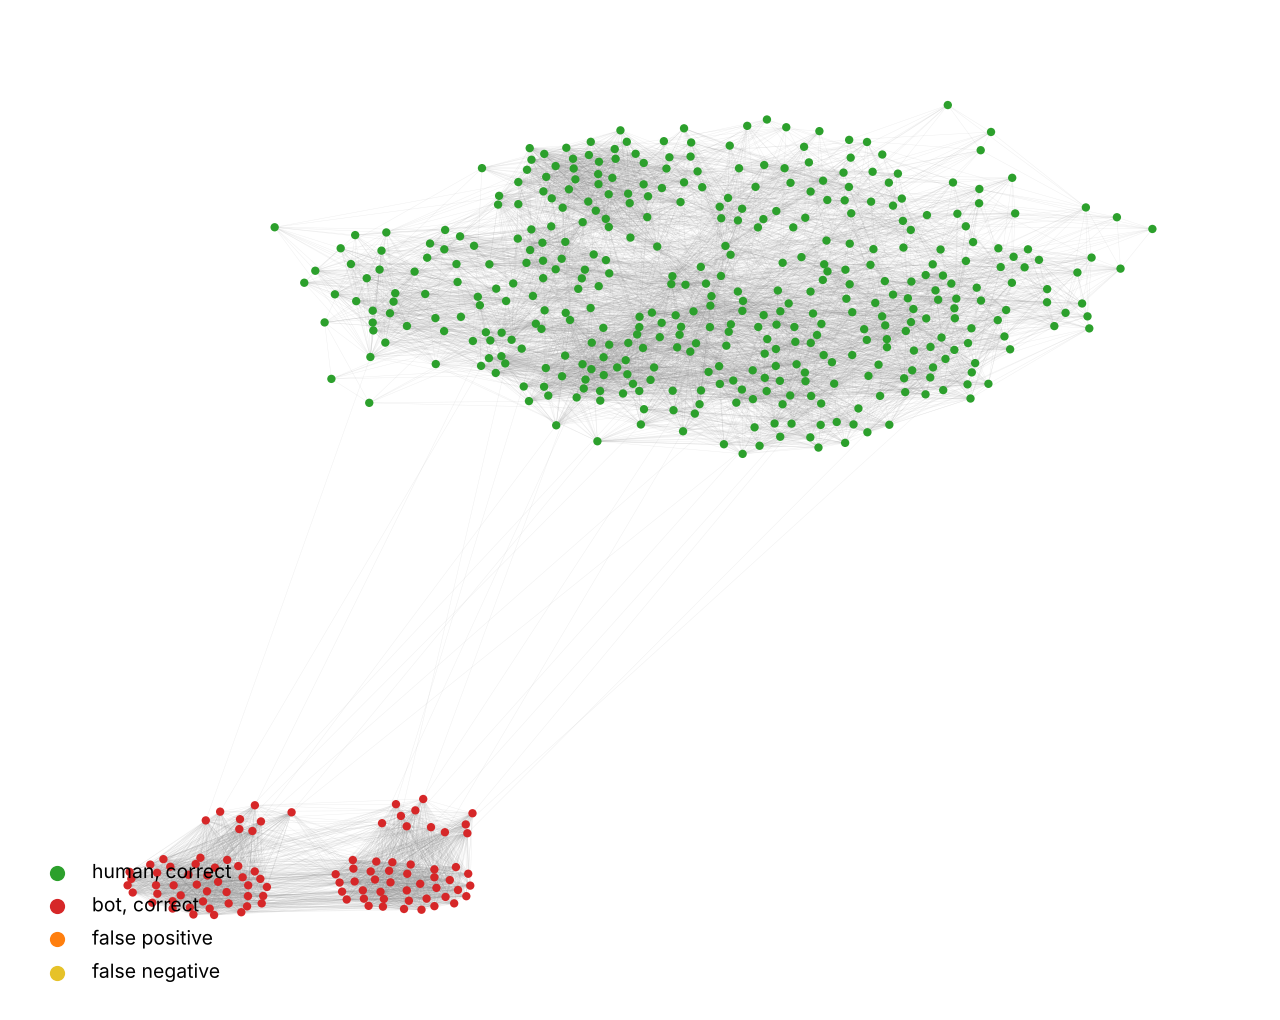
\includegraphics[width=0.92\columnwidth]{figures/fig1_synthetic_graph.png}
\caption{Synthetic graph (500 nodes, 10\,324 edges) colored by the Conf-GCN prediction: correctly classified humans (green) form a loose preferential-attachment community; correctly classified bots (red) form two dense, well-separated clusters. No node is misclassified.}
\label{fig:synthetic}
\end{figure}

Both models reach the task ceiling: accuracy, precision, recall and F1 are all 1.0000 for the baseline and the confidence-aware model (Table~\ref{tab:synthetic}, Fig.~\ref{fig:synthetic}); the same holds for MLP, GraphSAGE and GAT and for all 25 cross-validation runs of every model (125 runs, every metric 1.000). This is expected from the data-generating process: the bot clusters are fully connected subgraphs whose members share near-identical embeddings, producing a dense web of semantic edges within each cluster and almost none to the human subgraph, so the classes are separable by structure and by features alone. The task therefore verifies correctness (RQ1) but cannot discriminate between the models. Training loss falls to below $10^{-3}$ ($9.8\times10^{-4}$ for GCN, $6.5\times10^{-4}$ for Conf-GCN) for both models, and the mean confidence of the confidence-aware model rises from 0.998 at epoch 20 to 0.999 at epoch 100 (Fig.~\ref{fig:conf}), showing that the mechanism converges as intended. The unit tests confirm the formal properties of Section~\ref{sec:props}, in particular exact equivalence to mean aggregation when $c\equiv1$.

\subsection{Preliminary single-split result}

\begin{table}[t]
\caption{Real Twitter data, single split, as reported in our earlier study \cite{kassymkhan2026conf}}
\label{tab:prelim}
\centering
\footnotesize
\begin{tabular}{@{}lccc@{}}
\toprule
Metric & Baseline & Conf.-Aware & $\Delta$\\
\midrule
Accuracy & 0.7150 & 0.7130 & $-$0.0020\\
Precision & 0.7002 & 0.7300 & $+$0.0298\\
Recall & 0.7520 & 0.6760 & $-$0.0760\\
F1-score & 0.7252 & 0.7020 & $-$0.0232\\
\bottomrule
\end{tabular}
\end{table}

Table~\ref{tab:prelim} reproduces the original single train/test split on a 5\,000-account subsample of the full 37\,438-account release \cite{kassymkhan2026conf}. The confidence-aware model improved precision by 2.98 points while recall fell by 7.60 points and F1 by 2.32 points; accuracy was essentially unchanged. On a single split, differences of this size cannot be separated from sampling noise, which is why the protocol of Section~\ref{sec:protocol} was added. Absolute numbers below are not directly comparable with Table~\ref{tab:prelim} because the English-only redistribution yields a different subsample.

\subsection{Extended comparison (RQ2)}

\begin{table*}[t]
\caption{Real Twitter data (description $k$-NN graph, $k=10$), 5-fold CV $\times$ 5 seeds (mean $\pm$ std over 25 runs). $p$: paired Wilcoxon vs.\ Conf-GCN, Holm-corrected over the four baselines.}
\label{tab:main}
\centering
\footnotesize
\begin{tabular}{@{}lcccccccc@{}}
\toprule
Model & Acc. & Prec. & Rec. & F1 & AUROC & AUC-PR & $p$ (F1) & $p$ (Prec.)\\
\midrule
\tabinput{tables/table_main.tex}
\bottomrule
\end{tabular}
\end{table*}

Table~\ref{tab:main} shows the cross-validated comparison. Three findings stand out. First, the precision gain of Table~\ref{tab:prelim} does not replicate: Conf-GCN and GCN have the same mean precision (0.732 vs.\ 0.731, $p=0.83$). The recall loss does replicate in direction ($-2.0$ points), so Conf-GCN has a lower F1 than GCN (0.731 vs.\ 0.740, $p=0.004$) and is statistically indistinguishable from GAT in F1. Second, the threshold-independent metrics are clearly worse for Conf-GCN: AUROC 0.794 vs.\ 0.819 for GCN and GAT, AUC-PR 0.772 vs.\ 0.824, i.e.\ its ranking of accounts is worse, not merely shifted. Third, and most importantly for interpreting any GNN result on this benchmark, the feature-only MLP is the best model (F1 0.807, AUROC 0.890), tied with GraphSAGE (F1 0.803), whose separate root transformation lets it fall back on a node's own features. Models that mix a node's representation with its description neighbors (GCN, GAT, Conf-GCN) lose 6.7--7.6 F1 points relative to ignoring the graph. The run-to-run standard deviation of F1 (0.016--0.019 for GCN-type models) is of the same order as the single-split differences in Table~\ref{tab:prelim}, which explains why a single split was misleading.

\subsection{Ablations (RQ3)}

\begin{table}[t]
\caption{Ablations, description graph (mean $\pm$ std over 25 runs). $p$: paired Wilcoxon of F1 vs.\ full Conf-GCN, Holm-corrected over the nine comparisons.}
\label{tab:ablation}
\centering
\scriptsize
\setlength{\tabcolsep}{2.5pt}
\resizebox{\columnwidth}{!}{%
\begin{tabular}{@{}lccccc@{}}
\toprule
Variant & Prec. & Rec. & F1 & AUROC & $p$ (F1)\\
\midrule
\tabinput{tables/table_ablation.tex}
\bottomrule
\end{tabular}}
\end{table}

Table~\ref{tab:ablation} isolates the confidence signal. The uniform-confidence control, which keeps the layer but discards confidence, is \emph{at least as good} as the full model (F1 0.736 vs.\ 0.731, AUROC 0.795 vs.\ 0.794). Shuffled confidence, which preserves the marginal distribution but destroys node identity, and inverted weighting, which favors the \emph{least} confident neighbors, both land within 0.5 F1 points of the full model and are not significantly different from it. Sharpening the weights does not help either: $\alpha=2$ and $\alpha=4$ slightly lower F1 (0.728, 0.727) and AUROC (0.793, 0.788). The behavior of Conf-GCN is therefore explained by its normalization, not by confidence.

The self-loop variants identify which part of the normalization matters. Adding a self-loop to the uniform layer recovers GCN-level performance (F1 0.742, AUROC 0.817 vs.\ GCN 0.740, 0.819); adding it to the confidence-weighted layer recovers the AUROC (0.815) but not the F1 (0.734). The 2.5-point AUROC gap between Conf-GCN and GCN in Table~\ref{tab:main} is thus almost entirely due to the missing self-loop, i.e.\ to the node's own features being diluted by its neighbors. We answer RQ3 negatively: on this benchmark the confidence signal itself has no measurable benefit, and the precision-oriented behavior suggested by the single split is not a property of the method.

\subsection{Threshold-matched precision}

\begin{table}[t]
\caption{Test precision of each baseline at a threshold tuned on its validation set to Conf-GCN's validation recall (mean $\pm$ std over 25 runs). $\Delta$ = Conf-GCN $-$ baseline; $p$: paired Wilcoxon, Holm-corrected.}
\label{tab:threshold}
\centering
\scriptsize
\setlength{\tabcolsep}{2.5pt}
\begin{tabular}{@{}lccccc@{}}
\toprule
Baseline & Rec.\ (base) & Prec.\ (base) & Prec.\ (Conf) & $\Delta$ & $p$\\
\midrule
\tabinput{tables/table_threshold.tex}
\bottomrule
\end{tabular}
\end{table}

\begin{figure}[t]
\centering
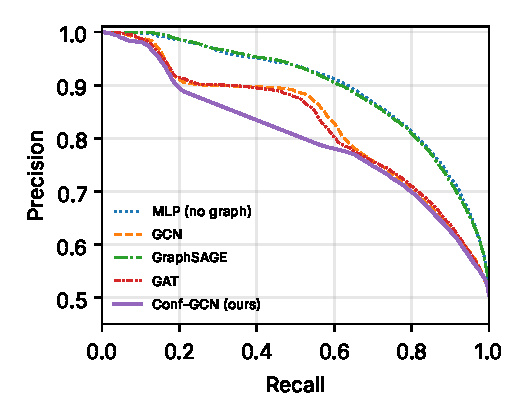
\includegraphics[width=\columnwidth]{figures/fig_pr_curves.pdf}
\caption{Precision--recall curves on the test folds (precision interpolated on a common recall grid and averaged over the 25 runs). Description graph, $k=10$.}
\label{fig:pr}
\end{figure}

Table~\ref{tab:threshold} asks whether a practitioner who wants Conf-GCN's operating point could obtain it more cheaply by moving the threshold of a baseline. At matched recall (0.730--0.733 for all models) GCN is 0.9 points and GAT 1.2 points \emph{more} precise than Conf-GCN, and MLP and GraphSAGE are about 12 points more precise; all differences are consistent across runs ($p<0.001$). The precision--recall curves (Fig.~\ref{fig:pr}) show the same picture at every operating point: the Conf-GCN curve lies below GCN and GAT, which lie well below MLP and GraphSAGE. Any precision-oriented operating point is therefore better obtained by raising the threshold of a baseline.

\subsection{Graph construction and density (RQ4)}

\begin{table}[t]
\caption{Effect of graph construction ($k=10$, mean $\pm$ std over 25 runs). Description graph: homophily 0.617; feature graph: 0.756.}
\label{tab:graph}
\centering
\scriptsize
\setlength{\tabcolsep}{2.5pt}
\begin{tabular}{@{}lcccc@{}}
\toprule
& \multicolumn{2}{c}{Description graph} & \multicolumn{2}{c}{Feature graph}\\
\cmidrule(lr){2-3}\cmidrule(lr){4-5}
Model & F1 & AUROC & F1 & AUROC\\
\midrule
\tabinput{tables/table_graph.tex}
\bottomrule
\end{tabular}
\end{table}

The description graph is a weak structure: only 61.7\% of its edges join accounts of the same class (50\% would be random for a balanced sample), and the 30\% of accounts with an empty description share an identical embedding, so their neighborhoods are essentially arbitrary among themselves. Building the $k$-NN graph over descriptions \emph{and} metadata raises edge homophily to 75.6\% and changes the conclusions (Table~\ref{tab:graph}): every GNN gains 2--9 F1 points ($p<10^{-6}$ for each), and all of them now beat the feature-only MLP (GraphSAGE 0.825, GCN 0.820, Conf-GCN 0.818, GAT 0.814 vs.\ 0.807; $p\le0.001$ for GCN, GraphSAGE and Conf-GCN, $p=0.001$ for GAT, unadjusted). On this better graph Conf-GCN is statistically tied with GCN in F1 (0.818 vs.\ 0.820, $p=0.12$) and precision (0.831 vs.\ 0.838, $p=0.08$), with a small but consistent AUROC deficit (0.901 vs.\ 0.905, $p<0.001$); confidence weighting does not become beneficial when the graph is more homophilous.

Graph density matters much less than graph construction. On the description graph, GCN reaches F1 0.732/0.740/0.734 for $k=5/10/20$ and Conf-GCN 0.729/0.731/0.726; GCN is ahead of Conf-GCN at every $k$ (unadjusted $p=0.15$, 0.002, $<0.001$).

\subsection{Why the confidence signal has no effect}
\label{sec:diag}

\begin{figure*}[t]
\centering
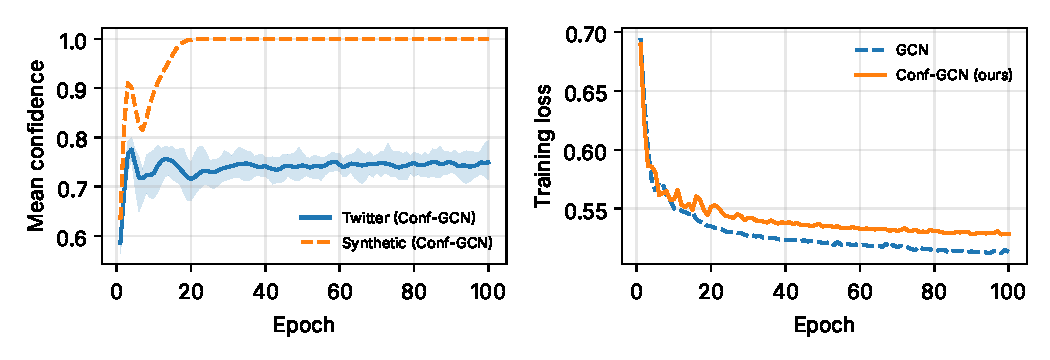
\includegraphics[width=0.85\textwidth]{figures/fig_confidence.pdf}
\caption{Left: mean confidence of Conf-GCN over training (real data: mean and min--max range over 25 runs; synthetic: single run). Right: mean training loss of GCN and Conf-GCN on the real data.}
\label{fig:conf}
\end{figure*}

We trained Conf-GCN on the five folds of seed~0 and inspected the final confidence vector and the resulting edge weights. Averaged over the 25 main runs, the mean confidence on the real data rises only from 0.586 after the first epoch to 0.749 at epoch 100 (Fig.~\ref{fig:conf}), in contrast to the synthetic graph where it saturates near 0.999; the 10th and 90th percentiles of the final confidences are 0.572 and 0.903. Inside a neighborhood the largest weight is a median 1.45$\times$ the smallest (95th percentile 1.82$\times$), and the weights deviate from uniform $1/\deg(i)$ by only 6.5\% on average. The bounded-influence property of Section~\ref{sec:props} therefore binds in practice: the layer is very close to mean aggregation, which is why the uniform control reproduces it. The confidence signal is also only moderately informative: as a score for whether a test node is classified correctly it reaches an AUROC of only 0.66 (0.77 on the feature graph, where the weights still deviate from uniform by just 7.1\%), and the softmax outputs of Conf-GCN are not better calibrated than those of the baselines (ECE 0.041 vs.\ 0.034 for GCN and 0.033 for MLP). Sharpening the weights with $\alpha>1$ amplifies this partly wrong signal and lowers AUROC (Table~\ref{tab:ablation}). The cost of the mechanism is a second forward pass per epoch; on a shared two-core CPU a Conf-GCN run (100 epochs) took 16.9\,s on average vs.\ 14.3\,s for GCN.

\section{Discussion}

\subsection{Answers to the research questions}
\textbf{RQ1:} the layer is correct: it converges on the synthetic graph, reduces exactly to mean aggregation for equal confidences, and has the same parameter count as GCN. \textbf{RQ2:} on the real data Conf-GCN does not improve any metric over GCN; it is equal in precision and worse in recall, F1, AUROC and AUC-PR, and all GCN-type models are beaten by an MLP on the description graph. \textbf{RQ3:} the differences from GCN are explained by the change of normalization (mean aggregation without self-loop), not by confidence: uniform, shuffled and inverted confidences behave like the full model, and a threshold-tuned GCN dominates it at matched recall. \textbf{RQ4:} graph construction dominates the aggregation rule; a more homophilous feature graph lifts every GNN above the MLP, but it does not make confidence weighting useful.

\subsection{Precision--recall trade-off and practical significance}
In moderation pipelines false positives are often more costly than false negatives: incorrectly labeling a genuine user as a bot can trigger restrictions and complaints, whereas a missed bot may be caught on a later pass as more interaction data accumulates. Under such an asymmetric cost structure a precision gain can be valuable even at the cost of recall. This argument was the motivation for the method, but it requires that the precision gain cannot be obtained more cheaply. Our threshold-matched analysis shows that it can: raising the threshold of GCN, or better of GraphSAGE or the MLP, gives higher precision at the same recall. The precision--recall trade-off observed in Table~\ref{tab:prelim} is therefore best interpreted as split noise around a different operating point, and we withdraw the ``implicit regularizer'' interpretation proposed in our earlier study.

\subsection{Absolute accuracy}
The best models reach about 81--83\% accuracy on balanced data using profile metadata and description text only, without tweet history or an explicit follow graph. Reported accuracy for comparable feature sets varies widely across datasets and protocols \cite{yang2020scalable,lee2021discriminative}, so we avoid claiming a specific literature band and instead rely on the in-paper MLP, GCN, GraphSAGE and GAT comparisons.

\subsection{Threats to validity}
\label{sec:threats}
\textbf{Graph construction:} the $k$-NN graphs are derived from the same embeddings (and, for the feature graph, the same metadata) used as features, so edges encode similarity already present in the features; real follow or mention graphs may behave differently. \textbf{Labels:} partly derived from Botometer, which is itself a feature-based detector, so metadata-based models may be favored. \textbf{Data:} we used an English-only cleaned redistribution and a 5\,000-account subsample; the code also accepts the original release. \textbf{Statistics:} runs share data across folds and seeds, so Wilcoxon $p$-values are indicative. \textbf{Hyper-parameters:} the grid is small and was selected on seed~0; all ablations reuse the Conf-GCN setting. \textbf{Bounded weights:} the binary confidence range restricts how far the mechanism can rebalance a neighborhood; multi-class problems or calibrated confidences may behave differently. \textbf{Confidence reliability:} softmax confidence is not guaranteed to be calibrated \cite{guo2017calibration}.

\section{Conclusion}
We presented a Confidence-Aware GCN that reweights neighbor contributions during message passing by each neighbor's own predictive confidence, recomputed every epoch and renormalized, with no additional learnable parameters. The mechanism is correct and cheap, but a rigorous evaluation on a real Twitter bot dataset shows that it does not deliver the precision gain suggested by an earlier single-split experiment: it ties GCN in precision, loses in recall, F1 and AUROC, and is dominated by a threshold-tuned GCN at matched recall. Controls with uniform, shuffled and inverted confidence reproduce its behavior, and diagnostics show why: in the binary case the confidence weights stay within a few percent of mean aggregation. The decisive factor on this benchmark is instead the graph: with a description-only $k$-NN graph no GCN-type model beats a feature-only MLP, while a $k$-NN graph over descriptions and metadata lifts all GNNs above it. We hope these results, together with the released code and per-run data, help others avoid over-interpreting single-split gains of aggregation tweaks and draw attention to graph construction for tabular bot datasets.

\section{Future Work}
Several directions remain open. Because the weights are bounded, a stronger signal is needed for confidence to matter: a learnable exponent $\alpha$ ($w_{j\rightarrow i}\propto c_j^{\alpha}$), which recovers uniform aggregation at $\alpha=0$, or a margin- or entropy-based confidence after temperature scaling \cite{guo2017calibration}. Confidence could modulate learned attention in GAT \cite{velickovic2018gat} instead of replacing degree normalization, or be added on top of GCN's symmetric normalization with self-loops so that only the confidence signal differs from the baseline. Evaluation on multi-relational graphs with explicit follow, mention, reply and retweet edges such as TwiBot-20 \cite{feng2021twibot20}, and on heterogeneous architectures such as BotRGCN \cite{feng2021botrgcn} with per-relation confidence, would show whether the mechanism helps when the graph is real rather than similarity-derived. Finally, the link between confidence-weighted aggregation and pseudo-labeling suggests a self-training extension in which high-confidence predictions seed supervision on unlabeled nodes \cite{lee2013pseudo}.

\section*{Code and Data Availability}
All code, configurations, per-run results (CSV), predicted probabilities and the scripts that generate every table and figure in this paper are available at \url{https://github.com/solodancer235-star/confidence-aware-gcn-bot-detection}. The full protocol runs on a two-core CPU in about two hours.

\section*{Acknowledgment}
The author thanks the School of Software Engineering at Astana IT University for guidance throughout the design and evaluation of this work.

\begin{thebibliography}{99}
\bibitem{kipf2017gcn} T. N. Kipf and M. Welling, ``Semi-supervised classification with graph convolutional networks,'' in \emph{Proc. ICLR}, 2017.
\bibitem{velickovic2018gat} P. Veli\v{c}kovi\'c, G. Cucurull, A. Casanova, A. Romero, P. Li\`o, and Y. Bengio, ``Graph attention networks,'' in \emph{Proc. ICLR}, 2018.
\bibitem{hamilton2017sage} W. L. Hamilton, R. Ying, and J. Leskovec, ``Inductive representation learning on large graphs,'' in \emph{Proc. NeurIPS}, 2017.
\bibitem{davis2016botornot} C. A. Davis, O. Varol, E. Ferrara, A. Flammini, and F. Menczer, ``BotOrNot: A system to evaluate social bots,'' in \emph{Proc. 25th Int. Conf. Companion on World Wide Web}, 2016, pp. 273--274.
\bibitem{yang2020scalable} K.-C. Yang, O. Varol, P.-M. Hui, and F. Menczer, ``Scalable and generalizable social bot detection through data selection,'' in \emph{Proc. AAAI}, vol. 34, no. 1, 2020, pp. 1096--1103.
\bibitem{cresci2020decade} S. Cresci, ``A decade of social bot detection,'' \emph{Commun. ACM}, vol. 63, no. 10, pp. 72--83, 2020.
\bibitem{alhosseini2019detect} S. Ali Alhosseini, R. Bin Tareaf, P. Najafi, and C. Meinel, ``Detect me if you can: Spam bot detection using inductive representation learning,'' in \emph{Companion Proc. World Wide Web Conf.}, 2019, pp. 148--153.
\bibitem{feng2021botrgcn} S. Feng, H. Wan, N. Wang, and M. Luo, ``BotRGCN: Twitter bot detection with relational graph convolutional networks,'' in \emph{Proc. IEEE/ACM ASONAM}, 2021.
\bibitem{feng2021twibot20} S. Feng, H. Wan, N. Wang, J. Li, and M. Luo, ``TwiBot-20: A comprehensive Twitter bot detection benchmark,'' in \emph{Proc. 30th ACM CIKM}, 2021, pp. 4485--4494.
\bibitem{feng2022rgt} S. Feng, Z. Tan, R. Li, and M. Luo, ``Heterogeneity-aware Twitter bot detection with relational graph transformers,'' in \emph{Proc. AAAI}, vol. 36, no. 4, 2022, pp. 3977--3985.
\bibitem{lee2021discriminative} D. Lee, S. Lee, and H. Yu, ``Discriminative feature selection for multi-class Twitter bot detection,'' \emph{IEEE Access}, vol. 9, pp. 32752--32762, 2021.
\bibitem{vashishth2019confgcn} S. Vashishth, P. Yadav, M. Bhandari, and P. Talukdar, ``Confidence-based graph convolutional networks for semi-supervised learning,'' in \emph{Proc. AISTATS}, 2019.
\bibitem{lee2013pseudo} D.-H. Lee, ``Pseudo-label: The simple and efficient semi-supervised learning method for deep neural networks,'' in \emph{ICML Workshop on Challenges in Representation Learning}, 2013.
\bibitem{guo2017calibration} C. Guo, G. Pleiss, Y. Sun, and K. Q. Weinberger, ``On calibration of modern neural networks,'' in \emph{Proc. ICML}, 2017, pp. 1321--1330.
\bibitem{rong2020dropedge} Y. Rong, W. Huang, T. Xu, and J. Huang, ``DropEdge: Towards deep graph convolutional networks on node classification,'' in \emph{Proc. ICLR}, 2020.
\bibitem{reimers2019sbert} N. Reimers and I. Gurevych, ``Sentence-BERT: Sentence embeddings using Siamese BERT-networks,'' in \emph{Proc. EMNLP}, 2019, pp. 3982--3992.
\bibitem{zhu2003semi} X. Zhu, Z. Ghahramani, and J. Lafferty, ``Semi-supervised learning using Gaussian fields and harmonic functions,'' in \emph{Proc. ICML}, 2003, pp. 912--919.
\bibitem{demsar2006statistical} J. Dem\v{s}ar, ``Statistical comparisons of classifiers over multiple data sets,'' \emph{J. Mach. Learn. Res.}, vol. 7, pp. 1--30, 2006.
\bibitem{kingma2015adam} D. P. Kingma and J. Ba, ``Adam: A method for stochastic optimization,'' in \emph{Proc. ICLR}, 2015.
\bibitem{fey2019pyg} M. Fey and J. E. Lenssen, ``Fast graph representation learning with PyTorch Geometric,'' in \emph{ICLR Workshop on Representation Learning on Graphs and Manifolds}, 2019.
\bibitem{gutierrez2021twitter} D. M. Guti\'errez, ``Twitter human bots dataset,'' Kaggle, 2021. [Online]. Available: \url{https://www.kaggle.com/datasets/davidmartngutirrez/twitter-bots-accounts}
\bibitem{botani2024} Bot-Ani project, ``Processed Twitter human/bot dataset (English accounts),'' GitHub, 2024. [Online]. Available: \url{https://github.com/Max-SF1/Bot-Ani-RWKV-twitter-bot-detection}
\bibitem{zhu2020beyond} J. Zhu, Y. Yan, L. Zhao, M. Heimann, L. Akoglu, and D. Koutra, ``Beyond homophily in graph neural networks: Current limitations and effective designs,'' in \emph{Proc. NeurIPS}, 2020.
\bibitem{holm1979simple} S. Holm, ``A simple sequentially rejective multiple test procedure,'' \emph{Scand. J. Statist.}, vol. 6, no. 2, pp. 65--70, 1979.
\bibitem{kassymkhan2026conf} K. Kassymkhan, ``Confidence-aware graph convolutional networks for social bot detection: A message-passing reweighting approach,'' in \emph{Proc. 2026 IEEE 3rd Int. Student Conf. on Digital Generation}, Astana, Kazakhstan, 2026.
\end{thebibliography}

\end{document}
